\chapter{Printed Circuit Board}

\glspl{pcb} play an essential role in this project. Breadboards and other prototyping techniques tend to cause issues with parasitic inductances and capacitances and do not work with \gls{smd} components, so \glspl{pcb} were the only way to build up the circuits. Once a \gls{pcb} has been produced, it works reliable and usually does not add any erratic effects. On the downside, however, \glspl{pcb} take a lot of time to design, etch, and solder, and once they are manufactured, they are very inflexible. This means that a new \gls{pcb} had to be made for every prototype..

\section{Component Selection}

Because almost none of the needed components were on hand in the school laboratories, they had to be ordered online. Due to the unique requirements of some parts, like the MOSFET or the \gls{vco}, they were rather hard to find and either very costly or came in an impractical package.

Since all the essential components were only available as \glspl{smd}, most other components were also shifted to \gls{smt} for consistency.


\subsection{ICs}

Most ICs were only available in one package and did not leave much flexibility. The MOSFET driver, \gls{vco}, latch, AND gate, and MOSFET for the phototransistor came in standard SOT and SOIC packages which were easy to solder since they have the pins on their side. The class-E MOSFET and the voltage regulator were somewhat troublesome because their packages had a big metal area on the underside, only indented for one-time reflow soldering. Unfortunately, the class-E MOSFET still needed to be replaced multiple times during the testing process. % flipflop & RUM

\subsection{Passive Elements}

All capacitors and resistors have been ordered in a 0805 package because it is not too big but just big enough to be easy to work with. The small size compared to \glspl{thd} does, however, negatively affect the power rating of resistors and the voltage rating of capacitors, so it had to be made sure that they still operated within the safe operating range. For the capacitors, X7R devices had been chosen, which means that their operating temperature ranges from -55\textdegree C to 125\textdegree C with at most 15\% capacitance change over this range\textsuperscript{\sidecite{epci}}. % potentiometer

\subsection{Peripherals}

To provide the necessary power and lead the MIDI-Interrupter signal to the \gls{pcb} as well as the ability to be turned on and off without being plugged out, one side of the \gls{pcb} enclosure has been dedicated as a control panel. % Possibly wordy sentence
For the power, a 5.5 x 2.1 mm barrel plug was used because of its widespread usage. To connect the fiber optic cable, the phototransistor has been mounted directly into the casing, so it is still accessible from the outside. Additionally, a keyswitch\sidenote{This way, only authorized people are able to turn on the Tesla coil and feel important} is used to turn on the power, and an ON-OFF-ON switch either routes the output of the phototransistor for interrupted operation, a constant 12V signal for continuous operating, or a 0V signal for no operation to the interrupt input.

\subsection{Miscellaneous Parts}

Since the four peripheral components cannot be mounted directly on the \gls{pcb}, because of its placement they had to be connected via wires. To cleanly organize those connections and be able to efficiently disconnect them all at once, a 6-pin connector was used. The single strands of the flat ribbon cable were then separated to connect to the switches and plugs.

A fuse was added on the Vcc rail to protect the circuit and the power supply from overcurrent. To save space and adhere to the \gls{smd}-only strategy, a 1206 package was used.

The boost converter for the 12\,V to 50\,V conversion was a tricky and very costly part. There were only very few parts for the desired voltage range and most of them were designed for hundreds of watts and came with a corresponding price tag. The final decision fell on the \emph{PKE3316HPI} from \emph{Flex Power Modules} which costs \emph{only} 33\,€.

% connectors to coil

\begin{tabular}{@{}lll@{}}
    \toprule
    \textbf{Part name} & \textbf{Footprint} & \textbf{Description}\\\midrule
    BSC12DN20N & PG-TDSON-8 & MOSFET\\
    IX4310 & SOT-23 & MOSFET driver\\
    LTC1799 & SOT-23 & Oscillator\\
    LM7805 & TO252 & Voltage regulator\\
    PKE3316 & Custom THT & boost converter\\
    74HC72 & SOIC127 & D-type latch\\
    TC7SZ08F & SOT-32 & AND gate\\
    RUM001L02 & SOT-723 & MOSFET\\
    47\(\mu\)H choke & Custom SMD &\\
    Various Capacitors & 0805 &\\
    Various Resistors & 0805 &\\
    Potentiometers & PT-10&\\
    Fuse 250mA & 1206 &\\
    Clamp & ? &\\
    \bottomrule
\end{tabular}

\section{Wiring}

\subsection{Peripherals}

\subsection{Coil connection}

\section{PCB Layout}

\begin{figure}[h!]
    \centering
    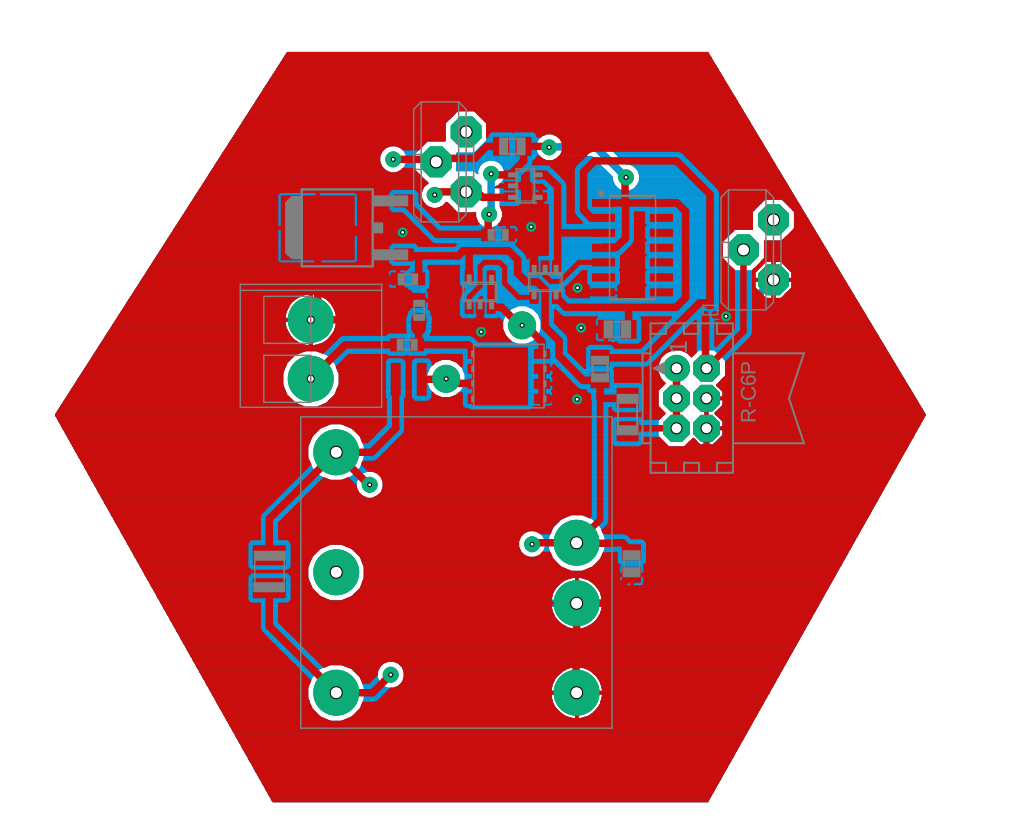
\includegraphics[width=\textwidth]{kassandra/resources/Tesla6Final.PNG}
    \caption{Final PCB Layout}
    \label{fig:tesla_layout}
\end{figure}

\subsection{Ground Planes}

\subsection{High Frequency Stuff}

\section{Manufacturing}

\subsection{Exposure}

\subsection{Stripping and Etching}

\subsection{Reflow Soldering}